\chapter{Genetika Populasi dan Seleksi Alam}\label{ch:b2:population-genetics}

Pada tahun 1848 seekor ngengat berbedak yang hitam ditangkap di dekat
Manchester; pada tahun 1895 sembilan belas dari dua puluh ngengat di
kotanya berwarna hitam, dan pada tahun 1970, ketika jelaganya pergi,
bentuk yang pucat kembali. Ngengatnya tidak berubah: perbandingan dua
\omterm{def:b2:meiosis-heredity:vocabulary}{alel} di dalam sebuah populasi berisi jutaan ekorlah yang berubah, di
bawah mata burung, dalam beberapa lusin generasi. Darwin telah melihat
bahwa seleksi pasti mengubah spesies tetapi tidak memiliki cara untuk
mencacahnya; pencacahannya adalah \omterm{def:b2:population-genetics:frequencies}{genetika populasi}, dan itulah
aritmetika bab ini. Bab ini menanyakan bagaimana \omterm{def:b2:population-genetics:frequencies}{frekuensi alel}
berperilaku ketika tidak ada yang bekerja padanya, lalu seberapa cepat
seleksi, \omterm{def:b2:genome-diversification:mutation}{mutasi}, migrasi, kebetulan, dan \omterm{prop:b2:population-genetics:inbreeding}{silang dalam} memindahkannya
--- dan bab ini berakhir dengan sifat yang bukan satu gen melainkan
banyak gen, yang merupakan sebagian besar dari yang sungguh dilihat
seleksi.

\section{Lungkang gennya ketika diam}

\begin{definition}[Populasi, lungkang gen, frekuensi]\label{def:b2:population-genetics:frequencies}
\index{genetika populasi}\index{lungkang gen}\index{frekuensi alel}
Sebuah \emph{populasi} adalah sekelompok individu satu spesies yang
saling mengawini; \emph{lungkang gennya} adalah himpunan seluruh
\omterm{def:b2:meiosis-heredity:vocabulary}{alelnya}. Bagi sebuah lokus dengan dua \omterm{def:b2:meiosis-heredity:vocabulary}{alel} $A$ dan $a$ di dalam sebuah
populasi \omterm{def:b2:meiosis-heredity:meiosis}{diploid} berisi $N$ individu, \emph{frekuensi \omterm{def:b2:meiosis-heredity:vocabulary}{alelnya}} adalah
$p = (2N_{AA} +
N_{Aa})/2N$ dan $q = 1 - p$, dan \emph{frekuensi
\omterm{def:b2:meiosis-heredity:vocabulary}{genotipenya}} adalah bagian $AA$, $Aa$, dan $aa$. Evolusi, dalam
pengertian yang paling sempit, adalah sebuah perubahan frekuensi \omterm{def:b2:meiosis-heredity:vocabulary}{alel}
antargenerasi; pertanyaan bab ini adalah apa yang mengubahnya dan
seberapa besar.
\end{definition}

\begin{theorem}[Hardy--Weinberg]\label{thm:b2:population-genetics:hw}
\index{hukum Hardy--Weinberg}
Di dalam sebuah populasi besar yang mengawin secara acak, tanpa
seleksi, \omterm{def:b2:genome-diversification:mutation}{mutasi}, atau migrasi, \omterm{def:b2:population-genetics:frequencies}{frekuensi alelnya} tidak berubah dari
satu generasi ke generasi berikutnya, dan setelah satu generasi
perkawinan acak frekuensi \omterm{def:b2:meiosis-heredity:vocabulary}{genotipenya} adalah
\[
AA : p^{2}, \qquad Aa : 2pq, \qquad aa : q^{2},
\]
lalu tetap demikian. Kedominanan tidak membuat sebuah \omterm{def:b2:meiosis-heredity:vocabulary}{alel} \omterm{def:b2:meiosis-heredity:vocabulary}{dominan}
menyebar, dan sebuah \omterm{def:b2:meiosis-heredity:vocabulary}{alel} \omterm{def:b2:meiosis-heredity:vocabulary}{resesif} yang jarang tidak hilang: ia
bersembunyi di dalam \omterm{def:b2:meiosis-heredity:vocabulary}{heterozigot}, yang kalah banyak terhadap
\omterm{def:b2:meiosis-heredity:vocabulary}{homozigotnya} dengan perbandingan $2p/q$ berbanding satu --- bagi $q = 0.01$, dua ratus berbanding satu. Hukumnya adalah hipotesis nol
\omterm{def:b2:population-genetics:frequencies}{genetika populasi}: sebuah penyimpangan darinya pada sebuah populasi
yang nyata, atau sebuah perubahan $p$ antargenerasi, adalah tanda
tangan salah satu gaya di bawah ini.
\end{theorem}
\begin{proof}
Perkawinan acak adalah penyatuan gamet secara acak: sebuah gamet
membawa $A$ dengan peluang $p$ dan $a$ dengan peluang $q$, bebas dari
pasangannya, sehingga zigotnya menjadi $AA$ dengan peluang $p^{2}$,
$Aa$ dengan $2pq$, dan $aa$ dengan $q^{2}$. \omterm{def:b2:population-genetics:frequencies}{Frekuensi alel} pada
generasi berikutnya adalah $p' = p^{2} + \tfrac12(2pq) = p(p + q) = p$:
tak berubah. Karena frekuensi \omterm{def:b2:meiosis-heredity:vocabulary}{genotipenya} hanya bergantung pada $p$,
frekuensinya sama pada tiap generasi setelah yang pertama.
\end{proof}

\begin{example}[Membaca sebuah frekuensi]\label{ex:b2:population-genetics:cf}
Fibrosis kistik, yang \omterm{def:b2:meiosis-heredity:vocabulary}{resesif}, menimpa satu anak Eropa dari 2500:
$q^{2} = 1/2500$, $q = 0.02$, dan frekuensi pembawanya adalah $2pq
\approx 0.04$ --- satu orang dari 25 membawa sebuah \omterm{def:b2:meiosis-heredity:vocabulary}{alel} yang membunuh
\omterm{def:b2:meiosis-heredity:vocabulary}{homozigotnya}, dan \qty{98}{\%} salinan \omterm{def:b2:meiosis-heredity:vocabulary}{alelnya} duduk di dalam pembawa
yang sehat tempat seleksi tidak dapat melihatnya. Itulah sebabnya
sebuah \omterm{def:b2:meiosis-heredity:vocabulary}{alel} \omterm{def:b2:meiosis-heredity:vocabulary}{resesif} yang mematikan disingkirkan begitu lambat, dan
sebabnya rencana eugenik untuk melenyapkan penyakit \omterm{def:b2:meiosis-heredity:vocabulary}{resesif} dengan
memandulkan yang terkena tidak pernah dapat berhasil: aritmetika bagian
berikutnya memperlihatkan seberapa lambat.
\end{example}

\section{Seleksi}

\begin{definition}[Kebugaran]\label{def:b2:population-genetics:fitness}
\index{kebugaran}\index{koefisien seleksi}
\emph{Kebugaran} $w$ sebuah \omterm{def:b2:meiosis-heredity:vocabulary}{genotipe} adalah sumbangan keturunannya
yang nisbi kepada generasi berikutnya --- kesintasan sampai berbiak
kali kesuburannya, yang diskalakan sehingga \omterm{def:b2:meiosis-heredity:vocabulary}{genotipe} yang terbaik
memiliki $w = 1$. \emph{Koefisien seleksi} $s$ sebuah \omterm{def:b2:meiosis-heredity:vocabulary}{genotipe} adalah
kekurangannya, $w = 1 - s$. Kebugaran adalah sifat sebuah \omterm{def:b2:meiosis-heredity:vocabulary}{genotipe} di
dalam sebuah lingkungan, bukan sifat sebuah \omterm{def:b2:meiosis-heredity:vocabulary}{alel} pada dirinya sendiri:
\omterm{def:b2:meiosis-heredity:vocabulary}{alel} ngengat melanik memiliki $w > 1$ terhadap \omterm{def:b2:meiosis-heredity:vocabulary}{alel} yang pucat pada
\omterm{def:b2:plant-meristems:wood}{kulit kayu} yang berjelaga dan $w < 1$ pada lumut kerak.
\end{definition}

\begin{theorem}[Seleksi mengubah frekuensi alel]\label{thm:b2:population-genetics:selection}
\index{seleksi alam!persamaan}
Dengan \omterm{def:b2:population-genetics:fitness}{kebugaran} \omterm{def:b2:meiosis-heredity:vocabulary}{genotipe} $w_{AA}$, $w_{Aa}$, $w_{aa}$, \omterm{def:b2:population-genetics:fitness}{kebugaran}
reratanya adalah $\bar w = p^{2}w_{AA} + 2pq\,w_{Aa} + q^{2}w_{aa}$ dan
\omterm{def:b2:population-genetics:frequencies}{frekuensi alel} pada generasi berikutnya adalah
\[
p' = \frac{p^{2}w_{AA} + pq\,w_{Aa}}{\bar w}, \qquad
\Delta p = p' - p = \frac{pq\,\bigl[p(w_{AA} - w_{Aa}) + q(w_{Aa} - w_{aa})\bigr]}{\bar w}.
\]
Dua akibatnya. Pertama, $\Delta p$ sebanding dengan $pq$: seleksinya
paling cepat pada frekuensi menengah dan paling lambat ketika sebuah
\omterm{def:b2:meiosis-heredity:vocabulary}{alel} jarang atau nyaris terpancang --- hanya ada sedikit keragaman
untuk dikenainya. Kedua, terhadap sebuah \omterm{def:b2:meiosis-heredity:vocabulary}{alel} \omterm{def:b2:meiosis-heredity:vocabulary}{resesif} ($w_{AA} = w_{Aa} = 1$, $w_{aa} =
1 - s$) perubahannya adalah $\Delta q = -s\,pq^{2}/\bar w$, yang sebanding dengan $q^{2}$: sebuah \omterm{def:b2:meiosis-heredity:vocabulary}{alel} \omterm{def:b2:meiosis-heredity:vocabulary}{resesif}
yang jarang nyaris tak terlihat oleh seleksi, dan menyetengahkan
frekuensinya dari $0.01$ memerlukan kira-kira seratus generasi
sekalipun \omterm{def:b2:meiosis-heredity:vocabulary}{homozigotnya} mematikan. Sebuah \omterm{def:b2:meiosis-heredity:vocabulary}{alel} \omterm{def:b2:meiosis-heredity:vocabulary}{dominan} yang
menguntungkan menyebar cepat pada mulanya lalu tersendat pada
akhirnya, karena alasan yang sama.
\end{theorem}
\begin{proof}
Dari keturunannya, sebagian sebesar $p^{2}w_{AA}/\bar w$ adalah $AA$
dan $2pq\,w_{Aa}/\bar w$ adalah $Aa$ (frekuensi tiap \omterm{def:b2:meiosis-heredity:vocabulary}{genotipenya}
dibobot dengan \omterm{def:b2:population-genetics:fitness}{kebugarannya} lalu dinormalkan ulang); \omterm{def:b2:meiosis-heredity:vocabulary}{alel} $A$ di antara
keturunannya adalah seluruh yang pertama dan separuh yang kedua,
sehingga memberikan $p'$. Mengurangkan $p =
p\bar w/\bar w$ lalu
menguraikan $\bar w$ memberikan $\Delta p$. Bagi sebuah \omterm{def:b2:meiosis-heredity:vocabulary}{alel} \omterm{def:b2:meiosis-heredity:vocabulary}{resesif}
yang mematikan ($s = 1$): $q' = q^{2}\cdot 0 + pq$ dibagi $\bar w = 1 -
q^{2}$, sehingga $q' = q/(1 + q)$, karena itu $1/q' = 1/q + 1$ dan
setelah $t$ generasi $1/q_t = 1/q_0 + t$: dari $q_0 = 0.01$ menjadi
$0.005$ memerlukan $t = 100$.
\end{proof}

\begin{omfigure}
\begin{tikzpicture}
\begin{axis}[
  width=0.8\linewidth, height=6cm,
  axis x line=bottom, axis y line=left,
  xmin=0, xmax=150, ymin=0, ymax=1.05,
  xlabel={generasi}, ylabel={frekuensi alel yang disukai},
  xlabel style={font=\small, at={(axis description cs:0.5,-0.11)}, anchor=north},
  ylabel style={font=\small},
  tick label style={font=\small}, xtick={0,50,100,150}, ytick={0,0.5,1},
  legend style={font=\scriptsize, at={(0.97,0.35)}, anchor=east, draw=none},
  clip=false,
]
\addplot[very thick, omDef] table[x=t, y=dom] {
t dom
0 0.01
10 0.02
20 0.04
30 0.075
40 0.14
50 0.24
60 0.38
70 0.53
80 0.66
90 0.76
100 0.83
110 0.88
120 0.91
130 0.93
140 0.945
150 0.955
};
\addlegendentry{alel yang disukai dominan, $s = 0.1$}
\addplot[very thick, omThm] table[x=t, y=rec] {
t rec
0 0.01
10 0.0101
20 0.0102
30 0.0104
40 0.0106
50 0.0108
60 0.011
70 0.0113
80 0.0116
90 0.012
100 0.0124
110 0.0128
120 0.0133
130 0.0138
140 0.0144
150 0.015
};
\addlegendentry{alel yang disukai resesif, $s = 0.1$}
\end{axis}
\end{tikzpicture}

{\small Seleksi ketika bekerja dengan keunggulan \qty{10}{\%}. Sebuah
\omterm{def:b2:meiosis-heredity:vocabulary}{alel} \omterm{def:b2:meiosis-heredity:vocabulary}{dominan} yang disukai naik dari \qty{1}{\%} menjadi mayoritas dalam
tujuh puluh generasi lalu melambat, sementara saingan \omterm{def:b2:meiosis-heredity:vocabulary}{resesifnya} yang
jarang bersembunyi di dalam \omterm{def:b2:meiosis-heredity:vocabulary}{heterozigot}; sebuah \omterm{def:b2:meiosis-heredity:vocabulary}{alel} \omterm{def:b2:meiosis-heredity:vocabulary}{resesif} yang
disukai pada \qty{1}{\%} nyaris tidak bergerak dalam waktu yang sama,
karena ia hampir tidak pernah tersingkap.}
\end{omfigure}

\begin{proposition}[Macam seleksi]\label{prop:b2:population-genetics:kinds}
\index{seleksi berarah}\index{seleksi pemantap}%
\index{seleksi penyeimbang}\index{keunggulan heterozigot}
Seleksi \emph{berarah} menyukai satu ujung lalu menggerakkan sebuah
\omterm{def:b2:meiosis-heredity:vocabulary}{alel} menuju fiksasi (ngengat melanik di dalam hutan yang berjelaga;
ketahanan antibiotika; ukuran paruh seekor burung pipit ketika
kekeringan). Seleksi \emph{pemantap} menyukai bagian tengahnya lalu
menyingkirkan ujungnya (bobot lahir manusia: bayi yang mati adalah yang
terkecil dan yang terbesar); ia menjaga sebuah populasi tetap di
tempatnya dan merupakan macam yang paling lazim. Seleksi
\emph{pemecah} menyukai kedua ujungnya terhadap bagian tengahnya, dan
dapat membelah sebuah populasi (\cref{ch:b2:speciation}). Seleksi
\emph{penyeimbang} menjaga dua \omterm{def:b2:meiosis-heredity:vocabulary}{alel} tetap berada di dalam populasinya
tanpa batas: lewat \emph{\omterm{prop:b2:population-genetics:kinds}{keunggulan heterozigot}}, ketika $Aa$ lebih
bugar daripada kedua \omterm{def:b2:meiosis-heredity:vocabulary}{homozigotnya} --- dengan $w_{AA} = 1 - s$, $w_{aa} = 1 - t$, $w_{Aa} = 1$, frekuensinya mengendap pada $\hat p = t/(s + t)$ --- atau lewat seleksi yang \emph{bergantung frekuensi}, ketika
sebuah \omterm{def:b2:meiosis-heredity:vocabulary}{genotipe} lebih bugar semakin jarang ia (\omterm{def:b2:meiosis-heredity:vocabulary}{alel} $S$ yang jarang
pada \cref{ch:b2:angiosperm-reproduction}, mangsa yang belum dipelajari
seekor pemangsa, dua sisi mulut seekor ikan pemakan sisik).
\end{proposition}
\begin{proof}[Bukti eksperimental]
Hemoglobin sel sabit membunuh sebagian besar \omterm{def:b2:meiosis-heredity:vocabulary}{homozigotnya} sebelum
mereka berbiak, namun \omterm{def:b2:meiosis-heredity:vocabulary}{alelnya} berada pada \qty{10}{\%} sampai
\qty{20}{\%} di seluruh Afrika yang bermalaria. Allison (1954)
menunjukkan bahwa anak yang \omterm{def:b2:meiosis-heredity:vocabulary}{heterozigot} mengalami jauh lebih sedikit
dan lebih ringan penularan malarianya daripada kedua \omterm{def:b2:meiosis-heredity:vocabulary}{homozigotnya}, dan
\omterm{def:b2:population-genetics:frequencies}{frekuensi alelnya} memetakan sebaran sejarah malaria falciparum; pada
populasi keturunan Afrika yang tinggal di tempat yang tidak bermalaria
frekuensinya terus turun sejak itu. Dengan $t \approx 0.8$ bagi
\omterm{def:b2:meiosis-heredity:vocabulary}{homozigot} sabitnya dan $s \approx 0.1$ bagi \omterm{def:b2:meiosis-heredity:vocabulary}{homozigot} normalnya di
sebuah daerah yang bermalaria, $\hat q = s/(s + t) \approx 0.11$ ---
itulah yang teramati.
\end{proof}

\section{Mutasi, migrasi, dan keseimbangannya}

\begin{theorem}[Keseimbangan mutasi--seleksi]\label{thm:b2:population-genetics:balance}
\index{keseimbangan mutasi--seleksi}\index{beban genetik}
Sebuah \omterm{def:b2:meiosis-heredity:vocabulary}{alel} yang merugikan disuapi \omterm{def:b2:genome-diversification:mutation}{mutasi} pada laju $\mu$ tiap gamet
tiap generasi lalu disingkirkan seleksi. Pada kesetimbangan keduanya
berimbang: bagi sebuah \omterm{def:b2:meiosis-heredity:vocabulary}{alel} \omterm{def:b2:meiosis-heredity:vocabulary}{resesif} dengan kerugian \omterm{def:b2:meiosis-heredity:vocabulary}{homozigot} $s$,
\[
\hat q = \sqrt{\mu/s}\,;
\]
bagi sebuah \omterm{def:b2:meiosis-heredity:vocabulary}{alel} \omterm{def:b2:meiosis-heredity:vocabulary}{dominan} (atau sebagian \omterm{def:b2:meiosis-heredity:vocabulary}{dominan}) dengan kerugian
\omterm{def:b2:meiosis-heredity:vocabulary}{heterozigot} $hs$, $\hat q = \mu/hs$. Karena itu frekuensi kesetimbangan
sebuah \omterm{def:b2:meiosis-heredity:vocabulary}{alel} \omterm{def:b2:meiosis-heredity:vocabulary}{resesif} besar bahkan bagi yang mematikan: dengan $\mu = 10^{-5}$ dan $s = 1$, $\hat q = 3\times 10^{-3}$, dan \qty{0.6}{\%}
populasinya membawanya. Tiap populasi membawa sebuah \emph{\omterm{thm:b2:population-genetics:balance}{beban
genetik}} semacam itu pada ribuan lokus, yang sebagian besarnya \omterm{def:b2:meiosis-heredity:vocabulary}{resesif}
dan tersembunyi, dan kesetimbangan hujah ratcet pada
\cref{ch:b2:asexual-reproduction} --- sebagian sebesar $e^{-U/s}$
individu yang bebas dari \omterm{def:b2:genome-diversification:mutation}{mutasi} yang merugikan --- adalah keseimbangan
yang sama yang dijumlahkan sepanjang genomnya.
\end{theorem}
\begin{proof}
Tiap generasi \omterm{def:b2:genome-diversification:mutation}{mutasinya} menambahkan $\mu p \approx \mu$ kepada $q$ dan
seleksinya menyingkirkan $s\,pq^{2}/\bar w \approx sq^{2}$ (bagi $q$
yang kecil); menetapkan $\mu = s\hat q^{2}$ memberikan hasil
\omterm{def:b2:meiosis-heredity:vocabulary}{resesifnya}. Bagi sebuah \omterm{def:b2:meiosis-heredity:vocabulary}{alel} \omterm{def:b2:meiosis-heredity:vocabulary}{dominan} seleksinya menyingkirkan $hs\,q$
tiap generasi (tiap salinannya tersingkap di dalam sebuah \omterm{def:b2:meiosis-heredity:vocabulary}{heterozigot}),
dan $\mu = hs\hat q$.
\end{proof}

\begin{proposition}[Migrasi dan kaidah satu migran]\label{prop:b2:population-genetics:migration}
\index{aliran gen}\index{migrasi (genetik)}
Jika sebagian sebesar $m$ dari sebuah populasi tiap generasinya adalah
pendatang dari sebuah populasi yang \omterm{def:b2:population-genetics:frequencies}{frekuensi alelnya} $p_{m}$,
frekuensinya berpindah menuju $p_{m}$ sebesar $\Delta p = m(p_{m} - p)$: selisih antara kedua populasinya meluruh sebagai $(1 - m)^{t}$.
\emph{\omterm{prop:b2:population-genetics:migration}{Aliran gen}} menyeragamkan; ia membatalkan \omterm{def:b2:plant-plasticity:plasticity}{adaptasi} setempat
kecuali jika seleksinya lebih kuat daripada $m$, dan ia adalah gaya
yang menjaga sebuah spesies tetap satu spesies. Sebaliknya, populasi
yang tidak bertukar migran memencar lewat hanyutan dan lewat \omterm{def:b2:genome-diversification:mutation}{mutasinya}
masing-masing, dan satu migran tiap generasi --- berapa pun ukuran
populasinya --- sudah cukup untuk mencegahnya menghanyut sampai
terpancang pada \omterm{def:b2:meiosis-heredity:vocabulary}{alel} yang berbeda.
\end{proposition}

\section{Kebetulan: hanyutan genetik}

\begin{theorem}[Hanyutan genetik]\label{thm:b2:population-genetics:drift}
\index{hanyutan genetik}\index{ukuran populasi efektif}\index{fiksasi}
Di dalam sebuah populasi berisi $N$ individu \omterm{def:b2:meiosis-heredity:meiosis}{diploid}, \omterm{def:b2:population-genetics:frequencies}{frekuensi alel}
tiap generasinya adalah sebuah contoh acak berisi $2N$ gamet dari
generasi sebelumnya, sehingga $p$ mengembara secara acak dengan ragam
$p(1 - p)/2N$ tiap generasi. \emph{Keheterozigotan} $H = 2pq$ meluruh
secara rerata dengan faktor $(1 - 1/2N)$ tiap generasi,
\[
H_t = H_0\left(1 - \frac{1}{2N}\right)^{t} \approx H_0\,e^{-t/2N},
\]
dan tiap \omterm{def:b2:meiosis-heredity:vocabulary}{alel} akhirnya hilang atau \emph{terpancang}, dengan peluang
yang sama dengan frekuensinya sekarang: sebuah \omterm{def:b2:genome-diversification:mutation}{mutasi} netral yang baru,
pada frekuensi $1/2N$, terpancang dengan peluang $1/2N$ dan, jika ia
terpancang, memerlukan kira-kira $4N$ generasi untuk mengerjakannya.
Hanyutannya dapat diabaikan pada sebuah populasi berisi jutaan dan
menguasai pada sebuah populasi berisi lusinan: sebuah \emph{leher
botol} atau sebuah peristiwa \emph{pendiri} --- beberapa penjajah di
sebuah pulau, sebuah spesies yang disusutkan menjadi seratus ekor oleh
perburuan --- kehilangan \omterm{def:b2:meiosis-heredity:vocabulary}{alel} secara kebetulan dalam satu generasi lalu
meninggalkan sebuah populasi yang seragam, miskin, dan penuh \omterm{def:b2:meiosis-heredity:vocabulary}{homozigot}.
Nilai $N$ yang berarti adalah ukuran \emph{efektifnya}, yaitu jumlah
individu yang sungguh berbiak, yang biasanya jauh lebih kecil daripada
cacah jiwanya.
\end{theorem}
\begin{proof}
Sebanyak $2N$ salinan gen generasi berikutnya diambil dengan
pengembalian dari sebuah lungkang yang di dalamnya $A$ berfrekuensi
$p$: jumlah salinan $A$-nya berdistribusi binomial dengan rerata $2Np$
dan ragam $2Np(1 - p)$, sehingga $p'$ memiliki rerata $p$ dan ragam
$p(1 - p)/2N$. Dua salinan yang diambil secara acak pada generasi
berikutnya berasal dari salinan induk yang sama dengan peluang $1/2N$
lalu menjadi serupa, sehingga peluang bahwa dua salinan berbeda (yaitu
keheterozigotannya) dikalikan $1 - 1/2N$ tiap generasi. Peluang
fiksasinya: frekuensi sebuah \omterm{def:b2:meiosis-heredity:vocabulary}{alel} netral adalah sebuah martingal ---
nilai harapannya tidak pernah berubah --- dan ia berakhir pada 0 atau
1, sehingga peluang berakhir pada 1 sama dengan nilai awalnya.
\end{proof}

\begin{omfigure}
\begin{tikzpicture}
\begin{axis}[
  width=0.82\linewidth, height=6cm,
  axis x line=bottom, axis y line=left,
  xmin=0, xmax=60, ymin=0, ymax=1.05,
  xlabel={generasi}, ylabel={frekuensi alel $p$},
  xlabel style={font=\small, at={(axis description cs:0.5,-0.11)}, anchor=north},
  ylabel style={font=\small},
  tick label style={font=\small}, xtick={0,20,40,60}, ytick={0,0.5,1},
  legend style={font=\scriptsize, at={(0.5,-0.25)}, anchor=north, draw=none, legend columns=2},
  clip=false,
]
\addplot[thick, omThm] coordinates {(0,0.5) (2,0.55) (4,0.62) (6,0.58) (8,0.7) (10,0.8) (12,0.75) (14,0.85) (16,0.92) (18,0.88) (20,0.95) (22,1) (60,1)};
\addlegendentry{$N = 10$}
\addplot[thick, omThm!60] coordinates {(0,0.5) (2,0.42) (4,0.35) (6,0.4) (8,0.3) (10,0.2) (12,0.25) (14,0.15) (16,0.1) (18,0.05) (20,0.08) (22,0.02) (24,0) (60,0)};
\addplot[thick, omDef] coordinates {(0,0.5) (5,0.52) (10,0.49) (15,0.53) (20,0.56) (25,0.54) (30,0.58) (35,0.55) (40,0.57) (45,0.6) (50,0.58) (55,0.61) (60,0.6)};
\addlegendentry{$N = 1000$}
\addplot[thick, omDef!60] coordinates {(0,0.5) (5,0.48) (10,0.5) (15,0.47) (20,0.45) (25,0.46) (30,0.44) (35,0.45) (40,0.43) (45,0.44) (50,0.42) (55,0.43) (60,0.42)};
\end{axis}
\end{tikzpicture}

{\small Hanyutan. Dua populasi berisi sepuluh individu yang bermula
pada $p = 0.5$ memancangkan \omterm{def:b2:meiosis-heredity:vocabulary}{alel} yang berlawanan dalam dua puluh lima
generasi; dua populasi berisi seribu individu mengembara beberapa
persen dalam enam puluh generasi.}
\end{omfigure}

\begin{proposition}[Silang dalam]\label{prop:b2:population-genetics:inbreeding}
\index{silang dalam}\index{koefisien silang dalam}\index{depresi silang dalam}
Perkawinan antarkerabat tidak mengubah \omterm{def:b2:population-genetics:frequencies}{frekuensi alelnya} tetapi
menaikkan bagian \omterm{def:b2:meiosis-heredity:vocabulary}{homozigotnya}: \emph{\omterm{prop:b2:population-genetics:inbreeding}{koefisien silang dalam}} $F$ sebuah
individu adalah peluang bahwa kedua \omterm{def:b2:meiosis-heredity:vocabulary}{alelnya} pada sebuah lokus serupa
menurut keturunan, dan frekuensi \omterm{def:b2:meiosis-heredity:vocabulary}{genotipenya} menjadi $p^{2} + Fpq$,
$2pq(1 - F)$, $q^{2} + Fpq$. Bagi keturunan sepupu pertama $F = 1/16$,
keturunan saudara kandung $1/4$, dan keturunan \omterm{def:b2:angiosperm-reproduction:pollination}{penyerbukan} sendiri
$1/2$. Karena \omterm{def:b2:meiosis-heredity:vocabulary}{alel} \omterm{def:b2:meiosis-heredity:vocabulary}{resesif} \omterm{thm:b2:population-genetics:balance}{beban genetiknya} tersingkap di dalam
\omterm{def:b2:meiosis-heredity:vocabulary}{homozigot} tambahannya, keturunan yang bersilang dalam menderita
\emph{\omterm{prop:b2:population-genetics:inbreeding}{depresi silang dalam}}: sebuah \omterm{def:b2:meiosis-heredity:vocabulary}{alel} \omterm{def:b2:meiosis-heredity:vocabulary}{resesif} yang mematikan pada $q = 0.01$ muncul pada $q^{2} = 10^{-4}$ keturunan yang kawin acak tetapi
pada $q^{2} + Fpq = 7\times 10^{-4}$ anak sepupu, yaitu tujuh kali
lebih banyak; jika dijumlahkan sepanjang ribuan lokus, anak sepupu
memiliki kira-kira dua kali kematian bayi orang lain, dan sebuah
populasi kecil yang bersilang dalam selama beberapa generasi kehilangan
kesuburan dan kegagahannya --- yaitu nasib citah, macan Florida, dan
wangsa raja Eropa.
\end{proposition}

\section{Banyak gen: sifat kuantitatif}

\begin{theorem}[Heritabilitas dan tanggapan terhadap seleksi]\label{thm:b2:population-genetics:heritability}
\index{heritabilitas}\index{genetika kuantitatif}\index{persamaan pemulia}
Sebuah sifat seperti tinggi, hasil, atau kedalaman paruh ditetapkan
oleh banyak gen yang efeknya kecil dan oleh lingkungannya, dan berubah
secara menerus. Ragamnya di dalam sebuah populasi terbelah menjadi
sebuah bagian \emph{genetik} $V_G$ dan sebuah bagian \emph{lingkungan}
$V_E$, dan \emph{heritabilitas} $h^{2} = V_A/V_P$ adalah bagian ragam
\omterm{def:b2:meiosis-heredity:vocabulary}{fenotipe} yang disebabkan efek aditif gennya (yaitu bagian yang
diturunkan). Jika induk generasi berikutnya diseleksi dengan sebuah
rerata yang melampaui rerata populasinya sebesar $S$ (yaitu
\emph{diferensial seleksi}), keturunannya melampauinya sebesar
\[
R = h^{2}\,S
\]
--- yaitu \emph{\omterm{thm:b2:population-genetics:heritability}{persamaan pemulia}}. Ia adalah seluruh pemuliaan hewan
dan tumbuhan dalam satu baris: heritabilitas $0.5$ dan induk yang satu
simpangan baku di atas reratanya memberikan keturunan yang setengah
simpangan baku di atasnya, dan perolehannya menimbun generasi demi
generasi. Heritabilitas adalah sifat sebuah populasi di dalam sebuah
lingkungan, bukan sifat sebuah karakter: ia tidak mengatakan apa pun
tentang apakah sebuah sifat terpancang, dan sebuah sifat dengan $h^{2} = 0.8$ pada satu populasi dapat memiliki $h^{2} = 0$ pada populasi lain
yang tiap individunya memiliki \omterm{def:b2:meiosis-heredity:vocabulary}{genotipe} yang sama.
\end{theorem}
\begin{proof}
\omterm{def:b2:meiosis-heredity:vocabulary}{Fenotipe} harapan keturunannya meregresi pada \omterm{def:b2:meiosis-heredity:vocabulary}{fenotipe} rerata kedua
induknya dengan kemiringan $h^{2}$ (yaitu peragam genetik aditif
antarkerabat dibagi ragam \omterm{def:b2:meiosis-heredity:vocabulary}{fenotipenya}), sehingga sebuah simpangan induk
$S$ memberikan sebuah simpangan keturunan $h^{2}S$. Dalam praktiknya
$h^{2}$ diukur dari regresi itu, atau dari kemiripan kembar dan saudara
kandung, atau dari tanggapannya sendiri.
\end{proof}
\begin{proof}[Bukti eksperimental]
Percobaan jagung Illinois, yang dimulai pada tahun 1896, menyeleksi
tongkol yang kandungan minyaknya tertinggi dan terendah tiap tahun:
setelah seratus generasi galur yang tinggi telah naik dari \qty{5}{\%}
menjadi \qty{20}{\%} minyak dan galur yang rendah telah turun sampai di
bawah \qty{1}{\%}, dan keduanya masih menanggapi --- keragaman banyak
gen tidak habis oleh satu abad seleksi. Di Galapagos, keluarga Grant
mengukur tiap burung pipit di satu pulau sepanjang kekeringan tahun
1977: yang bertahan hidup memiliki paruh yang \qty{4}{\%} lebih dalam
daripada yang mati, sifatnya memiliki $h^{2}
\approx 0.7$, dan anak
tahun berikutnya memiliki paruh yang \qty{3}{\%} lebih dalam daripada
paruh generasi sebelumnya --- seleksi yang teramati, terukur, dan
tanggapannya diramalkan persamaan di atas.
\end{proof}

\begin{omfigure}
\begin{tikzpicture}
\begin{axis}[
  width=0.78\linewidth, height=5.6cm,
  axis x line=bottom, axis y line=left,
  xmin=6, xmax=14, ymin=0, ymax=0.32,
  xlabel={kedalaman paruh (mm)}, ylabel={frekuensi},
  xlabel style={font=\small, at={(axis description cs:0.5,-0.12)}, anchor=north},
  ylabel style={font=\small},
  tick label style={font=\small}, xtick={7,9,11,13}, ytick=\empty,
  legend style={font=\scriptsize, at={(0.5,-0.28)}, anchor=north, draw=none, legend columns=3},
  clip=false,
]
\addplot[very thick, omDef, domain=6:14, samples=100] {0.3*exp(-((x-9.4)^2)/(2*0.9))};
\addlegendentry{sebelum kekeringannya, rerata 9.4}
\addplot[very thick, omThm, domain=6:14, samples=100] {0.28*exp(-((x-9.9)^2)/(2*0.8))};
\addlegendentry{yang bertahan hidup, rerata 9.9}
\addplot[very thick, omProp, dashed, domain=6:14, samples=100] {0.3*exp(-((x-9.75)^2)/(2*0.9))};
\addlegendentry{generasi berikutnya, rerata 9.75}
\draw[<->] (axis cs:9.4,0.02) -- (axis cs:9.9,0.02); \node[font=\scriptsize, anchor=south] at (axis cs:9.65,0.025) {$S$};
\end{axis}
\end{tikzpicture}

{\small \omterm{thm:b2:population-genetics:heritability}{Persamaan pemulia} pada sebuah populasi burung pipit.
Kekeringannya meninggalkan yang bertahan hidup dengan paruh rerata $S = \qty{0.5}{mm}$ lebih dalam; dengan $h^{2} = 0.7$ keturunannya
$R = \qty{0.35}{mm}$ lebih dalam daripada generasi sebelumnya.}
\end{omfigure}

\begin{example}[Aritmetika ngengatnya]\label{ex:b2:population-genetics:moth}
\omterm{def:b2:meiosis-heredity:vocabulary}{Alel} melanik ngengat berbedaknya bersifat \omterm{def:b2:meiosis-heredity:vocabulary}{dominan}. Dari sebuah
frekuensi kira-kira $10^{-3}$ pada tahun 1848 menjadi \qty{90}{\%}
ngengatnya (yaitu sebuah frekuensi mendekati $0.7$) pada tahun 1895
adalah lima puluh generasi; persamaan seleksinya menghasilkannya
kembali dengan $s$ antara $0.2$ dan $0.3$ terhadap bentuk yang pucat
--- dan percobaan pelepasan Kettlewell pada tahun 1950-an, yang di
dalamnya burung mengambil ngengat pucat dari batang yang berjelaga dan
ngengat gelap dari batang yang bersih dengan nisbah kira-kira sebesar
itu, mengukur koefisiennya secara langsung. Kembalinya setelah
undang-undang udara bersih, dari \qty{90}{\%} melanik pada tahun 1960
menjadi di bawah \qty{10}{\%} pada tahun 2000, berjalan pada kecepatan
yang sama ke arah yang lain. Seluruh peristiwanya --- sebuah populasi
besar, sebuah \omterm{def:b2:meiosis-heredity:vocabulary}{alel} \omterm{def:b2:meiosis-heredity:vocabulary}{dominan}, dan sebuah agen seleksi yang kuat dan dapat
balik --- adalah \omterm{def:b2:population-genetics:frequencies}{genetika populasi} yang terjadi di depan umum.
\end{example}

\begin{omfigure}
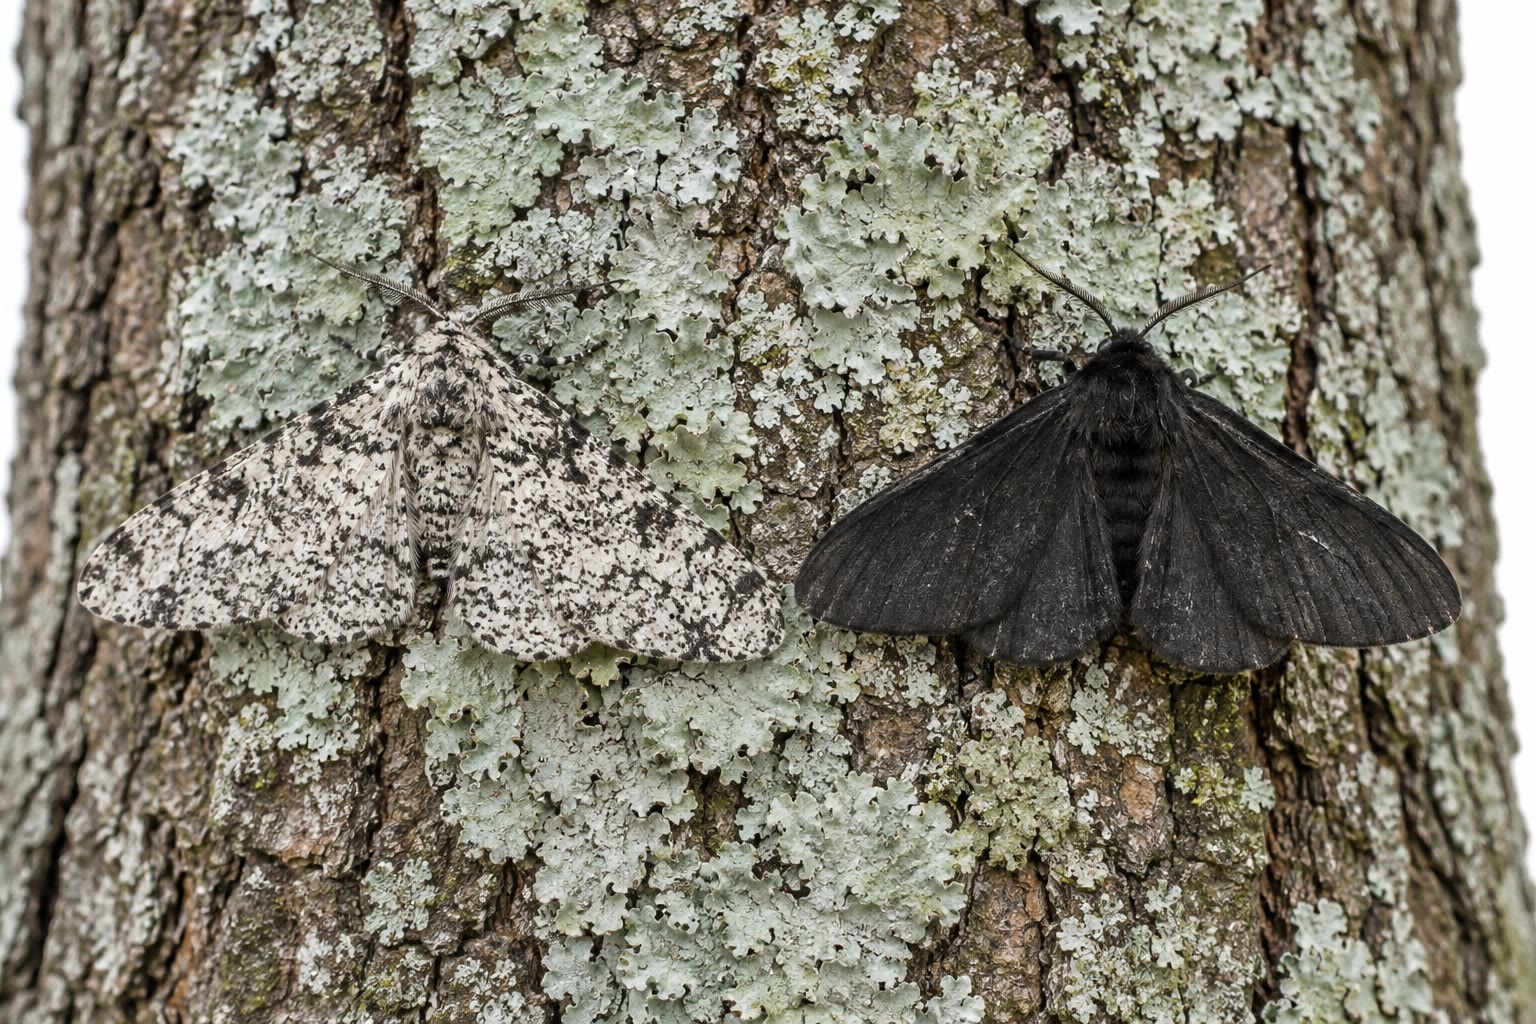
\includegraphics[width=0.46\linewidth]{images/book4/ai/b4-22-peppered-moths.jpg}\hspace{0.04\linewidth}
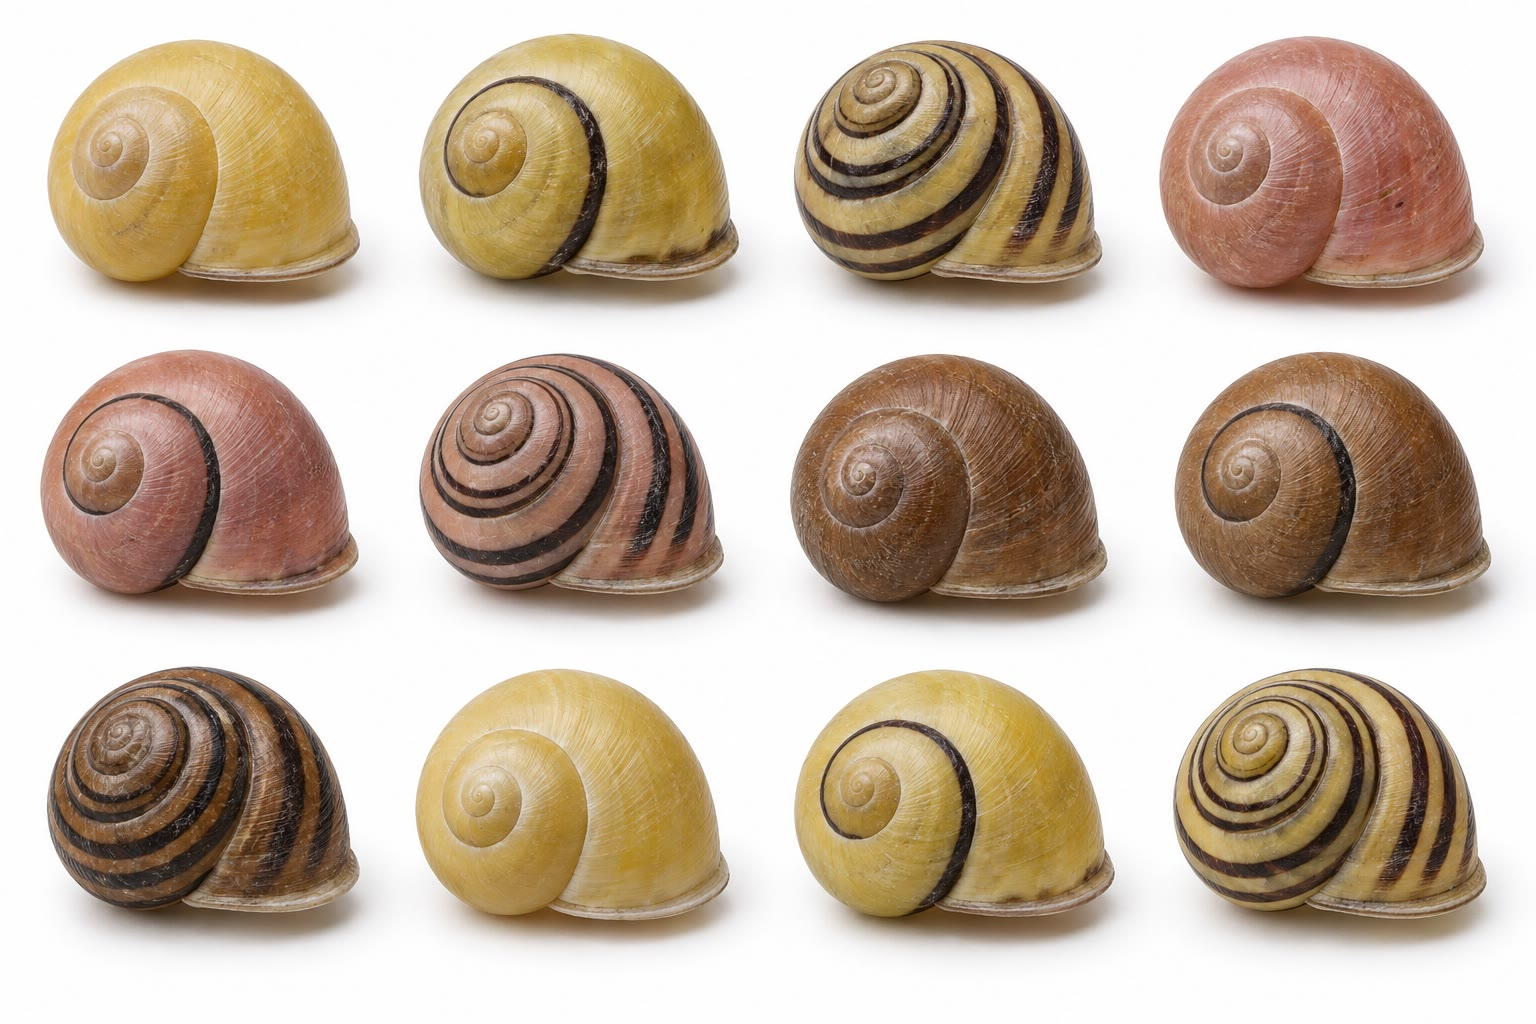
\includegraphics[width=0.46\linewidth]{images/book4/ai/b4-22-banded-snails.jpg}

{\small Kiri: kedua bentuk ngengat berbedaknya pada lumut kerak ---
yang mana yang ditemukan seekor burung bergantung pada \omterm{def:b2:plant-meristems:wood}{kulit kayunya}.
Kanan: polimorfisme cangkang siput hutan, dengan warna dan pita yang
dijaga tetap ada pada tiap populasinya oleh pemangsa yang mempelajari
bentuk yang lazim.}
\end{omfigure}

\section{Latihan}

\begin{exercise}[$\star$]\label{exo:b2:population-genetics:1}
Pada sebuah contoh berisi 1000 orang, 640 orang bergenotipe $MM$, 320
orang $MN$, dan 40 orang $NN$. Hitunglah \omterm{def:b2:population-genetics:frequencies}{frekuensi alelnya} dan harapan
Hardy--Weinbergnya. Apakah populasinya berada dalam kesetimbangan?
\end{exercise}

\begin{exercise}[$\star$]\label{exo:b2:population-genetics:2}
Albinisme bersifat \omterm{def:b2:meiosis-heredity:vocabulary}{resesif} dan menimpa satu orang dari \num{20000}.
Hitunglah \omterm{def:b2:population-genetics:frequencies}{frekuensi alelnya} dan frekuensi pembawanya.
\end{exercise}

\begin{exercise}[$\star$]\label{exo:b2:population-genetics:3}
Definisikan \omterm{def:b2:population-genetics:fitness}{kebugaran}, \omterm{def:b2:population-genetics:fitness}{koefisien seleksi}, dan heritabilitas, lalu
berikan kelima gaya yang mengubah \omterm{def:b2:population-genetics:frequencies}{frekuensi alel}.
\end{exercise}

\begin{exercise}[$\star$]\label{exo:b2:population-genetics:4}
Berikan satu contoh masing-masing bagi \omterm{prop:b2:population-genetics:kinds}{seleksi berarah}, \omterm{prop:b2:population-genetics:kinds}{seleksi
pemantap}, dan \omterm{prop:b2:population-genetics:kinds}{seleksi penyeimbang}, beserta agen seleksinya
masing-masing.
\end{exercise}

\begin{exercise}[$\star\star$]\label{exo:b2:population-genetics:5}
Sebuah \omterm{def:b2:meiosis-heredity:vocabulary}{alel} \omterm{def:b2:meiosis-heredity:vocabulary}{resesif} yang mematikan berfrekuensi $0.02$. Berapa generasi
untuk menyetengahkannya? Untuk mencapai $0.001$? Apa yang dikatakan hal
ini tentang efek mencegah individu yang terkena untuk berbiak?
\end{exercise}

\begin{exercise}[$\star\star$]\label{exo:b2:population-genetics:6}
Dengan $w_{AA} = 1$, $w_{Aa} = 1$, $w_{aa} = 0.8$, dan $p = 0.3$,
hitunglah $\bar w$, $p'$, dan $\Delta p$. Ulangi bagi $p = 0.9$.
Mengapa perubahan yang kedua jauh lebih kecil?
\end{exercise}

\begin{exercise}[$\star\star$]\label{exo:b2:population-genetics:7}
\omterm{def:b2:meiosis-heredity:vocabulary}{Homozigot} sel sabitnya memiliki $w = 0.2$ dan \omterm{def:b2:meiosis-heredity:vocabulary}{homozigot} normalnya $w = 0.88$ di sebuah daerah yang bermalaria, sedangkan \omterm{def:b2:meiosis-heredity:vocabulary}{heterozigotnya} $w = 1$. Hitunglah frekuensi kesetimbangan \omterm{def:b2:meiosis-heredity:vocabulary}{alel} sabitnya dan bagian anak
yang lahir dengan penyakitnya pada kesetimbangannya.
\end{exercise}

\begin{exercise}[$\star\star$]\label{exo:b2:population-genetics:8}
Sebuah \omterm{def:b2:meiosis-heredity:vocabulary}{alel} \omterm{def:b2:meiosis-heredity:vocabulary}{resesif} yang mematikan muncul lewat \omterm{def:b2:genome-diversification:mutation}{mutasi} pada $\mu = \qty{2e-5}{}$ tiap gamet. Hitunglah frekuensi kesetimbangannya dan
bagian kelahiran yang terkena. Sebuah \omterm{def:b2:meiosis-heredity:vocabulary}{alel} \omterm{def:b2:meiosis-heredity:vocabulary}{dominan} yang mematikan
(sebelum berbiak) pada laju yang sama: bagian kelahiran berapa?
\end{exercise}

\begin{exercise}[$\star\star$]\label{exo:b2:population-genetics:9}
Sebuah populasi berisi 50 individu yang berbiak bermula dengan $H = 0.5$. Hitunglah keheterozigotannya setelah 10, 50, dan 200 generasi.
Seberapa besar sebuah populasi harus dibuat untuk menjaga \qty{90}{\%}
keheterozigotannya sepanjang 100 generasi?
\end{exercise}

\begin{exercise}[$\star\star\star$]\label{exo:b2:population-genetics:10}
Sebuah pulau dijajah 10 ekor burung dari sebuah populasi daratan yang
di dalamnya sebuah \omterm{def:b2:meiosis-heredity:vocabulary}{alel} berfrekuensi $0.1$. Hitunglah peluang bahwa
\omterm{def:b2:meiosis-heredity:vocabulary}{alelnya} tidak ada pada pendirinya, dan peluang bahwa ia akhirnya
terpancang di pulaunya jika ia hadir dalam satu salinan. Bandingkan
dengan daratannya.
\end{exercise}

\begin{exercise}[$\star\star\star$]\label{exo:b2:population-genetics:11}
Hasil susu memiliki $h^{2} = 0.3$ dan simpangan baku \qty{1000}{L}.
Seorang pemulia menyimpan \qty{20}{\%} sapi teratas sebagai induk
(reratanya $1.4$ simpangan baku di atas rerata kawanannya). Hitunglah
tanggapannya tiap generasi. Jika pejantannya dipilih dari \qty{1}{\%}
teratas (rerata $2.7$ simpangan baku di atasnya), berapakah
tanggapannya? Mengapa tanggapannya melambat setelah banyak generasi?
\end{exercise}

\begin{exercise}[$\star\star\star$]\label{exo:b2:population-genetics:12}
``Seleksi buta terhadap apa yang tidak dapat ia lihat.'' Bahaslah,
dengan \omterm{def:b2:meiosis-heredity:vocabulary}{alel} \omterm{def:b2:meiosis-heredity:vocabulary}{resesif} di dalam \omterm{def:b2:meiosis-heredity:vocabulary}{heterozigot}, \omterm{def:b2:genome-diversification:mutation}{mutasi} netralnya, dan sifat
yang heritabilitasnya nol, apa yang dapat dan tidak dapat dikenai
seleksi.
\end{exercise}

\section{Soal: Ngengat, Pulau, dan Kawanan}

\begin{problem}[{Soal akhir pekan --- kenaikan ngengat berbedaknya
dihitung dari persamaan seleksi, hanyutan dan silang dalam sebuah
populasi pendiri diikuti, sebuah keseimbangan mutasi--seleksi
ditegakkan, dan sebuah program pemulia diramalkan, berakhir pada
koefisien seleksi ngengatnya, keheterozigotan pulaunya, dan perolehan
kawanannya}]
\label{pb:b2:population-genetics:1}
Ngengat berbedak: \omterm{def:b2:meiosis-heredity:vocabulary}{alel} melanik $M$ \omterm{def:b2:meiosis-heredity:vocabulary}{dominan}, berfrekuensi $p_0 = 0.001$
pada tahun 1848; \qty{90}{\%} ngengatnya melanik 50 generasi kemudian;
anggaplah $w_{MM} = w_{Mm} = 1$ dan $w_{mm} = 1 - s$. Pulaunya:
didirikan 12 ekor burung dari sebuah daratan yang $H = 0.4$ dan sebuah
\omterm{def:b2:meiosis-heredity:vocabulary}{alel} \omterm{def:b2:meiosis-heredity:vocabulary}{resesif} yang merugikan memiliki $q = 0.05$; pulaunya menampung 40
burung yang berbiak sesudahnya. \omterm{def:b2:genome-diversification:mutation}{Mutasi}: $\mu = \qty{1e-5}{}$.
Kawanannya: $h^{2} = 0.4$, simpangan baku \qty{800}{L}.

\medskip
\noindent\textbf{Bagian I --- Ngengatnya.}
\begin{enumerate}
  \item Pada tahun 1848, bagian ngengat berapa yang melanik, dan
        bagian \omterm{def:b2:meiosis-heredity:vocabulary}{alel} $M$ berapa yang duduk di dalam \omterm{def:b2:meiosis-heredity:vocabulary}{heterozigot}?
  \item Tunjukkan bahwa, dengan $M$ \omterm{def:b2:meiosis-heredity:vocabulary}{dominan}, \omterm{def:b2:population-genetics:frequencies}{frekuensi alel} yang pucat
        mematuhi $q' = q(1 - sq)/(1 - sq^{2})$.
  \item Bermula dari $q_0 = 0.999$, hitunglah $q$ setelah satu generasi
        bagi $s = 0.3$.
  \item Melanik \qty{90}{\%} berarti $q^{2} = 0.1$. Berapakah $q$
        ketika itu?
  \item Dengan mencoba-coba rekursinya (atau hampirannya
        $\Delta q \approx -sq^{2}p$ selama $q$ dekat 1), taksirlah
        jumlah generasi bagi $s = 0.3$ untuk membawa $q$ dari $0.999$
        menjadi $0.32$, lalu bandingkan dengan 50 yang teramati.
  \item Setelah undang-undang udara bersihnya bentuk yang pucat
        memiliki keunggulannya, sehingga $s
        = 0.3$ terhadap $mm$
        menjadi $s = 0.3$ terhadap $M\_$. Tunjukkan bahwa $\Delta p = -spq^{2}/\bar w$, lalu jelaskan mengapa kembalinya bentuk yang
        pucat lambat pada mulanya dan berakhir pada sebuah penurunan
        eksponensial $M$, sedangkan kenaikannya bermula secara
        eksponensial lalu berakhir dengan merangkak.
\end{enumerate}

\medskip
\noindent\textbf{Bagian II --- Pulaunya.}
\begin{enumerate}[resume]
  \item Hitunglah peluang bahwa tak seorang pun dari 12 pendirinya
        membawa \omterm{def:b2:meiosis-heredity:vocabulary}{alel} yang merugikan itu.
  \item Hitunglah keheterozigotan harapan setelah generasi
        pendiriannya (diambil dari $H = 0.4$ oleh 12 individu, yakni 24
        salinan gen).
  \item Hitunglah keheterozigotannya setelah 100 generasi pada $N =
        40$, sebagai bagian dari keheterozigotan daratannya.
  \item Sebuah \omterm{def:b2:genome-diversification:mutation}{mutasi} netral muncul pada seekor burung. Hitunglah
        peluang fiksasinya dan waktu harapan sampai fiksasinya jika ia
        terpancang.
  \item Burung pulaunya mengawin secara acak tetapi semuanya
        berkerabat. Dengan $F = 1/(2N)$ yang menimbun tiap generasi
        menjadi kira-kira $0.3$ setelah 30 generasi, hitunglah
        frekuensi \omterm{def:b2:meiosis-heredity:vocabulary}{homozigot} yang terkena bagi \omterm{def:b2:meiosis-heredity:vocabulary}{alelnya} pada $q = 0.05$,
        dengan dan tanpa \omterm{prop:b2:population-genetics:inbreeding}{silang dalamnya}.
  \item Seekor burung daratan tiba tiap generasi. Jelaskan apa yang
        dikerjakan hal ini terhadap pemencaran pulaunya dan bebannya.
\end{enumerate}

\medskip
\noindent\textbf{Bagian III --- Keseimbangannya.}
\begin{enumerate}[resume]
  \item Hitunglah frekuensi kesetimbangan sebuah \omterm{def:b2:meiosis-heredity:vocabulary}{alel} \omterm{def:b2:meiosis-heredity:vocabulary}{resesif} yang
        mematikan yang disuapi $\mu = 10^{-5}$, dan bagian kelahiran
        yang terkena.
  \item Hitunglah hal yang sama bagi $s = 0.1$ (sebuah \omterm{def:b2:meiosis-heredity:vocabulary}{alel} \omterm{def:b2:meiosis-heredity:vocabulary}{resesif}
        yang agak merugikan).
  \item Hitunglah kesetimbangannya bagi sebuah \omterm{def:b2:meiosis-heredity:vocabulary}{alel} \omterm{def:b2:meiosis-heredity:vocabulary}{dominan} dengan
        kerugian \omterm{def:b2:meiosis-heredity:vocabulary}{heterozigot} $hs = 0.05$.
  \item Kedokteran menyembuhkan yang mematikannya sehingga $s$ turun
        menjadi $0.1$. Bagaimana kesetimbangannya berubah, dan berapa
        lama (orde besarannya) populasinya memerlukan waktu untuk
        mencapainya?
  \item Genomnya memiliki \num{20000} gen yang masing-masing bermutasi
        menjadi sebuah \omterm{def:b2:meiosis-heredity:vocabulary}{alel} \omterm{def:b2:meiosis-heredity:vocabulary}{resesif} yang mematikan pada $10^{-5}$.
        Berapa banyak \omterm{def:b2:meiosis-heredity:vocabulary}{alel} mematikan yang dibawa seorang rerata dalam
        keadaan \omterm{def:b2:meiosis-heredity:vocabulary}{heterozigot}? (Pada kesetimbangannya tiap lokus memiliki
        $2\hat q$ salinan tiap orangnya.)
  \item Jelaskan mengapa jumlah itu selaras dengan sebuah populasi yang
        sehat dan mengapa ia membuat perkawinan sepupu berongkos mahal.
\end{enumerate}

\medskip
\noindent\textbf{Bagian IV --- Kawanannya.}
\begin{enumerate}[resume]
  \item Pemulianya menyimpan \qty{30}{\%} sapi teratas (reratanya
        $1.16$ simpangan baku di atas kawanannya). Hitunglah
        diferensial seleksinya dalam liter dan tanggapannya.
  \item Setelah lima generasi seleksi yang sama, berapakah perolehan
        harapannya, dan mengapa perolehan yang sebenarnya mungkin lebih
        kecil?
  \item Pejantannya menyumbang separuh gennya dan diseleksi dari
        \qty{2}{\%} teratas ($2.4$ simpangan baku). Hitunglah
        tanggapannya ketika sapi dan pejantannya diseleksi seperti di
        atas (reratakan kedua diferensialnya).
  \item Sebuah kawanan yang seluruh sapinya adalah klona satu ekor
        hewan: berapakah $h^{2}$ dan tanggapannya? Apa yang dikatakan
        hal itu tentang heritabilitas?
  \item Sebuah populasi burung pipit memiliki $h^{2} = 0.7$ bagi
        kedalaman paruhnya dan kekeringannya meninggalkan yang bertahan
        hidup \qty{0.6}{mm} lebih dalam. Ramalkan generasi berikutnya.
  \item Pemulianya beralih kepada sebuah sifat dengan $h^{2} = 0.1$.
        Diferensial seleksi berapa, dalam simpangan baku, yang
        memberikan tanggapan yang sama dengan pertanyaan 19?
  \item Nyatakan hasilnya: $s$ ngengatnya dan waktu sampai
        \qty{90}{\%} melanik, keheterozigotan pulaunya setelah 100
        generasi, dan tanggapan kawanannya tiap generasi.
\end{enumerate}
\end{problem}
